\documentclass[10pt, a4paper]{article}
\usepackage[utf8x]{inputenc}            % Acentos, ñ, etc.
\usepackage{graphicx}                   % Gráficos
\usepackage[spanish]{babel}             % Macros en español
\usepackage{caratula}                   % Carátula
\begin{document}

%Caratula
\titulo{Trabajo Práctico 1}
\subtitulo{Detección de Spam}
\fecha{\today}
\materia{Aprendizaje Automático}
\integrante{Fernández, Gonzalo}{836/10}{gpfernandezflorio@gmail.com}
\integrante{Damian, Aleman}{377/10}{damianealeman@gmail.com}
\integrante{Matías, Pizzagalli}{257/10}{matipizza@gmail.com}



%Titulo e indice
\maketitle
\tableofcontents
\newpage

\section*{Introducción}

%\includegraphics{algo.png}
\section{Metodología}
Cargamos los mails de los archivos json
Extrajimos los atributos de la base de mails y los guardamos como matrices
Separamos los datos de entrenamiento de los de test utilizando la funciøn train\_test\_split y almacenamos cada conjunto en archivos npy.

\section{Extracción de atributos}
%Describir en castellano los atributos extraidos de los mails, en forma concisa.
Para saber que palabras identifican mejor a los mails de spam, implementamos un script que cuenta la cantidad de ocurrencias por palabra, relativa entre los mails de spam contra los de ham.
Es decir, para cada palabra en los archivos json este script devuelve la cantidad de apariciones de dicha palabra en el archivo de spam menos la cantidad de apariciones de la misma palabra en el archivo ham.
Este script está implementado en el archivo \texttt{wordCounter.py}. En el archivo \texttt{words-100.txt} se pueden ver las 100 palabras con mayor cantidad de ocurrencias relativa.

En principio usamos como atributos la cantidad de apariciones de estas palabras en cada mail. Por otro lado agregamos los atributos

\begin{itemize}
\item Cantidad de palabras en mayusculas.
\item Cantidad de palabras compuestas por numeros.
\item Cantidad de palabras escritas con la primera letra en mayuscula.
\item Cantidad de letras promedio por palabra. 
\item Cantidad de letras maxima por palabra. 
\end{itemize}


\section{Modelos}
%Listar los algoritmos de aprendizaje elegidos para experimentar. Describir cualquier decisión que hayan tomado (p.ej., elección de hiperparámetros).
Utilizamos los siguientes algoritmos de aprendizaje:

\begin{itemize}
\item Decision Tree
\item Random Forest
\item Naive Bayes
\item Vecinos Más Cercanos(KNN)
\item Support Vector Machines (SVM)
\end{itemize}

\section{Reducción de dimensionalidad} 
Sobre técnicas de reducción de dimensionalidad usamos:

\begin{description}
\item PCA []
\item ICA
\item iPCA
\item REFCV[ Con esta ténica vimos los atributos que ofrecen mayor poder predictivo]
\end{description}

% Describir brevemente las técnicas empleadas.
\section{Resultados}
 %Describir los resultados conseguidos por los distintos modelos y conjuntos de atributos considerados. Preferentemente, resumir los resultados en tablas/figuras. Mencionar los tiempos de ejecución aproximados de cada técnica.

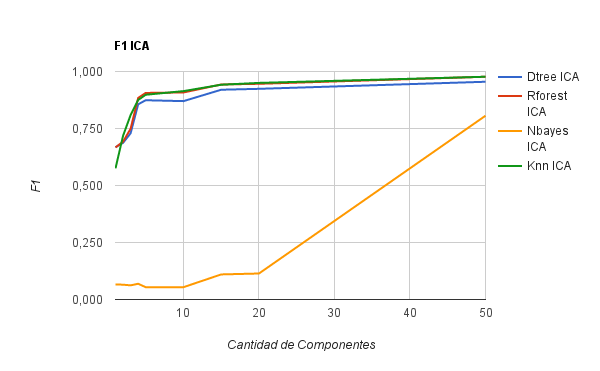
\includegraphics[width=\textwidth]{../imgs/F1ICA.png}
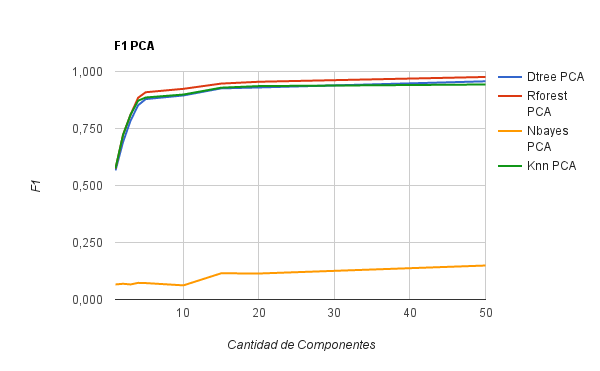
\includegraphics[width=\textwidth]{../imgs/F1PCA.png}
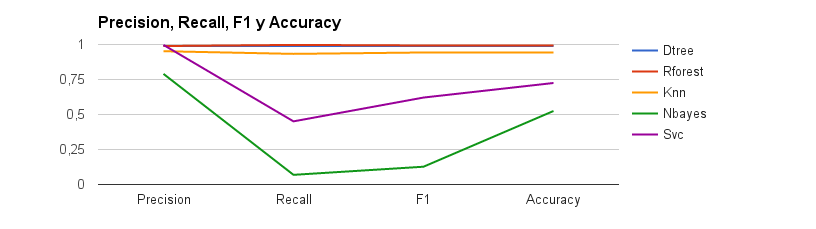
\includegraphics[width=\textwidth]{../imgs/metodos1.png}
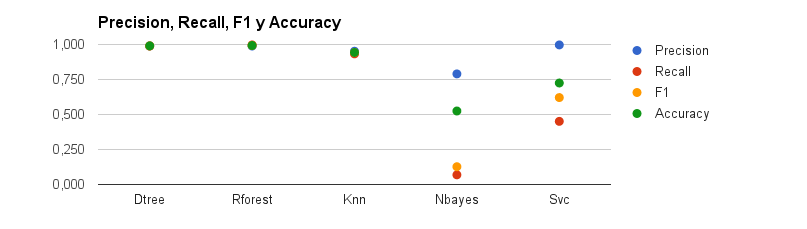
\includegraphics[width=\textwidth]{../imgs/metodos2.png}
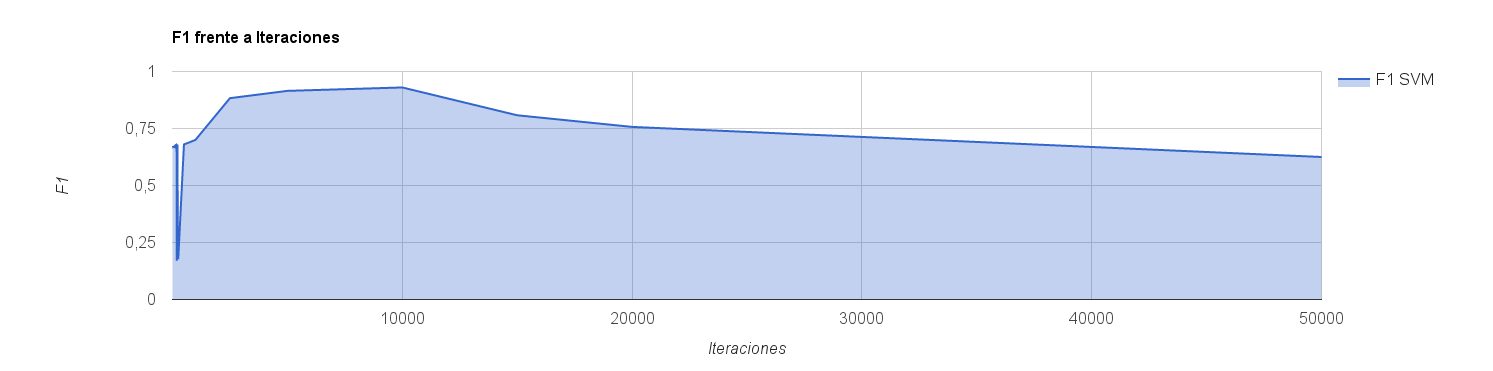
\includegraphics[width=\textwidth]{../imgs/SVCFULL.png}
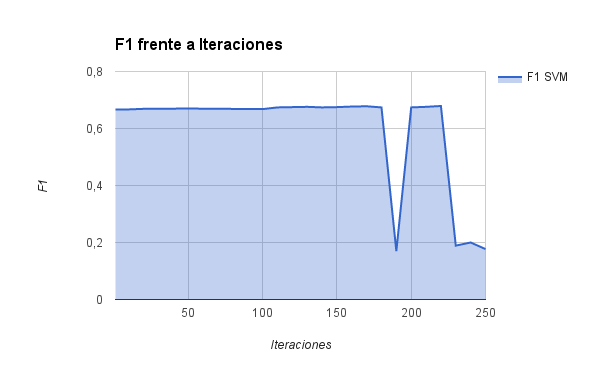
\includegraphics[width=\textwidth]{../imgs/SVCSTART.png}

% 
 
\section{Discusión}
 %Analizar los resultados, buscando responder cuestiones como, por ejemplo: ¿cuáles son los atributos encontrados con mayor poder predictivo?, ¿cuán sensibles fueron los algoritmos a las técnicas de reducción de dimensionalidad consideradas?, ¿resultó clara la elección del algoritmo para la competencia, o hubo que poner en la balanza distintos factores?
 
% A continuación podemos ver los atributos con mayor poder predictivo seleccionados con el metodo de RFCV

% Podemos ver un græfico con medidas de cuan bueno es un modelo con pocas componentes y como mejora a lo largo del incremento de componentes

\end{document}
